\chapter{Physical aspects}

Atomic nuclei have multiple energy states, many of which are not stable, forcing them to release some of their energy in order to reach a stable state. One decay however, does not always lead to a direct transition into a stable state, it may even require the atom to transform into another depending on what way it has released its energy by. The theory on this chapter regarding energy and particle emissions from decaying nuclei is based on the detailed information shown in the first chapters of ``Radiation Detection and Measurement'' by Glenn F. Knoll \cite{knoll2010radiation}. On the other hand, radiation is not only produced when atoms decay, it is constantly raining down upon us from the cosmos, this kind of radiation can also be detected with a CosmicWatch, making it also necessary to explore. This chapter aims to provide an overview of some of the mechanisms through which nuclei reach stable states and what cosmic radiation is. Chapter \ref{chap:detection_methods} provides an overview of how this can be used to take interesting measurements with CosmicWatch.

\section{Radioactivity}

It is first necessary to understand the concept of activity. Not all atoms take the same time to decay, each atom has its own constant $\Gamma$ which determines how likely it is to decay per unit of time. If one has an initial total of $N_0$ atoms, after a while it will be reduced due to the constant decay of atoms in the sample, this rate of change is given by the universal law of radioactive decay.
\begin{equation}
    \frac{dN(t)}{dt} = -\Gamma N(t)
\end{equation}

From this, it is easy to find that the number of remaining unstable atoms follows an exponential law
\begin{equation}
    N(t) = N_0 e^{-\Gamma t}
\end{equation}

The activity $A(t)$ of a radioactive source is given by how many decays occur per unit of time. This can be therefore obtained by multiplying the number of atoms $N(t)$ by the probability of decay per unit of time $\Gamma$.
\begin{equation}
    A(t) = \Gamma N_0 e^{-\Gamma t}
\end{equation}

The most common units for activity are the \textit{curie} (Ci) and the \textit{becquerel} (Bq), a becquerel represents one disintegration per second, while a curie represents $3.7\times10^{10}$ disintegrations per second ($\approx$ the activity of one gram of $^{226}Ra$). Under these definitions, the conversion between these units is given by the following relation:
\begin{eqnarray}
    1 \text{~Bq} = 2.703\times10^{-11} \text{~Ci}
\end{eqnarray}

The time constant $\Gamma$ is often expressed in terms of the atom's lifetime $\tau$ under the relation $\Gamma=1/\tau$. This means that $\tau$ is the time it takes to reduce a sample of $N_0$ by a factor of $1/e$, clearly $N(\tau)=N_0e^{-\Gamma \tau} = N_0/e$. On the other hand there also exists a constant called half-life $T_{1/2}$, which represents the time it takes to reduce the sample by half, Sodium 22 for example has a half-life of 2.605 years. They can both be related by doing $T_{1/2} = \ln (2)\tau$.

\subsection{Gamma emission}

\begin{figure}
  \centering
  \begin{subfigure}[t]{0.45\textwidth}
    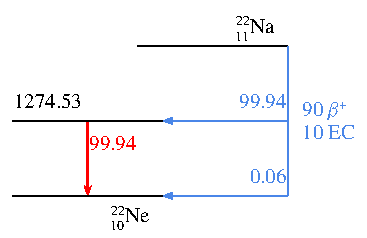
\includegraphics[width=\textwidth]{physical_aspects/22Na-decay.pdf}
    \caption{\label{sfig:22Na}}
  \end{subfigure}
  \begin{subfigure}[t]{0.425\textwidth}
    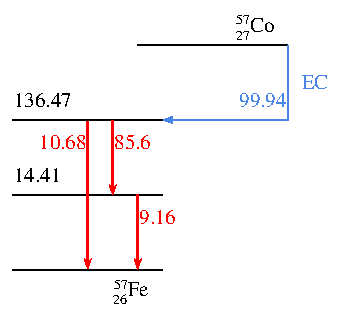
\includegraphics[width=\textwidth]{physical_aspects/57Co-decay.pdf}
    \caption{\label{sfig:57Co}}
  \end{subfigure}
  \medskip
  \centering
  \begin{subfigure}[t]{0.425\textwidth}
    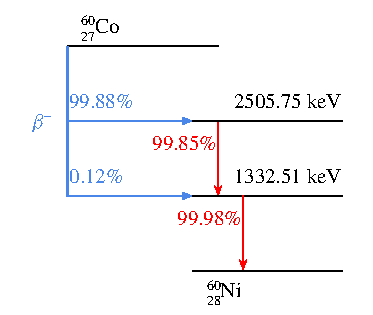
\includegraphics[width=\textwidth]{physical_aspects/60Co-decay.pdf}
    \caption{\label{sfig:60Co}}
  \end{subfigure}
  \begin{subfigure}[t]{0.425\textwidth}
    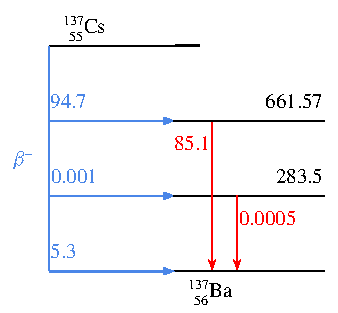
\includegraphics[width=\textwidth]{physical_aspects/137Cs-decay.pdf}
    \caption{\label{sfig:137Cs}}
  \end{subfigure}
  \caption{\label{fig:decay_schemes}Decay schemes for some isotopes used while testing the CosmicWatch. Only the main decay channels are included for clarity and simplicity. Energies [\unit{\kilo\eV}] for every level are shown in black. Branching ratios and decay mechanisms are shown in \textcolor{blue}{blue}. Gamma decays are represented with a \textcolor{red}{red} arrow also with its corresponding branching ratio.}
\end{figure}

Unstable nuclei have multiple channels to release their energy through, the conditions that determine what channels an atom can use are not studied here, but rather the subsequent effects of such channels. An atom can decay by emitting gamma rays, alpha particles, neutrons, or protons, it can also undergo beta $\beta^{\pm}$ decay, Internal Conversion, and Electron Capture among others. This work will focus on beta decay and Electron Capture since these are the preferred channels of decay of the radioactive sources used to test CosmicWatch.

\subsubsection{Beta decay}

There are two types of beta decay, they are represented by the following reaction schemes:
\begin{align}
  \beta^+ &:=~ ^A_ZX \rightarrow ~ ^A_{Z-1}Y + e^+ + \nu \\
  \beta^- &:=~ ^A_ZX \rightarrow ~ ^A_{Z+1}Y + e^- + \bar{\nu}
\end{align}

Where the symbols follow the nuclear notation, $X$ and $Y$ represent the initial and final elements, $A$ is the atomic number, $Z$ the nuclear charge, $e^{\pm}$ are a positron or electron, and $\nu/\bar{\nu}$ are a neutrino/antineutrino, Fig. \ref{fig:decay_schemes} shows some examples of these processes. Note for instance the case of $^{22}_{11}$Na Fig. \ref{sfig:22Na}, it undergoes $\beta^+$ $90\%$ of the time it decays, by the nuclear notation one can tell that the initial and final elements are Sodium and Neon respectively. In this process, a proton turns into a neutron, which is why the product element has $Z=11-1=10$ while maintaining $A=22$. It is important to also note that the total charge has to be conserved after the reaction occurs, which is why a positron $e^+$ is produced.

Alongside the positron/electron, a neutrino/antineutrino is ejected from the nucleus which, due to its extremely small interaction probability with matter, can not be detected. However, the negligible neutrino/antineutrino-matter interactions do not mean that their presence in the reaction does not have effects. The energy of the system also has to be conserved, since the particles $e^{\pm}$ and $\nu/\bar{\nu}$ are all ejected from the nucleus, higher or smaller portions of the total energy can be taken by the neutrino/antineutrino, which leaves multiple possible energy values for the positron/electron, resulting in continuous energy spectra.

\begin{figure}[H]
    \centering
    \begin{subfigure}[t]{0.45\textwidth}
      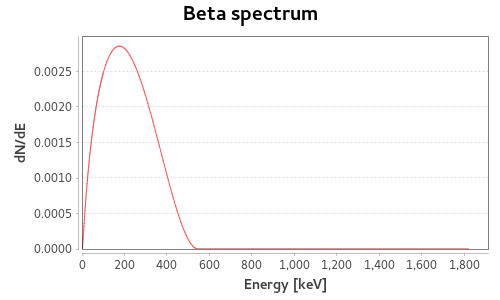
\includegraphics[width=\textwidth]{physical_aspects/22Na-beta-spectrum.jpg}
      \caption{\label{sfig:22Na_beta_spectra}}
    \end{subfigure}
    \begin{subfigure}[t]{0.45\textwidth}
      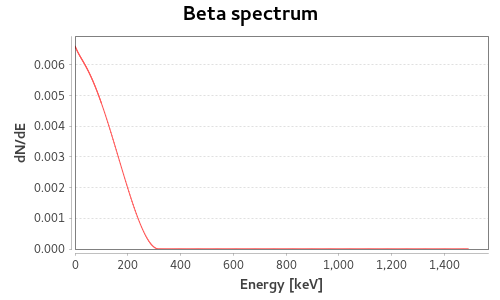
\includegraphics[width=\textwidth]{physical_aspects/60Co-beta-spectrum.jpg}
      \caption{\label{sfig:60Co_beta_spectra}}
    \end{subfigure}
    \caption{\label{fig:beta_spectra}positron/electron energy spectra for  \subref{sfig:22Na_beta_spectra} $^{22}$Na $(\beta^+)$ and  \subref{sfig:60Co_beta_spectra} $^{60}$Co $(\beta^-)$. Taken from \cite{IAEA}.}
\end{figure}

\subsubsection{Electron Capture}

The process of Electron Capture is analogous to $\beta^+$ decay, here an electron from de $K$ shell (or $L$, $M$, \dots) is captured by a proton in the nucleous, which then turns into a neutron while emitting a neutrino with a characteristic energy. The effect of this decay in the nucleous is the same as in $\beta^+$: (Z, A)$\rightarrow$(Z-1, A). The decay scheme is represented below:

\begin{equation}
  \text{EC} :=~ p + e^- \rightarrow ~ n + \nu
\end{equation}

Since this process leaves a vacancy in the lower shells of the electron cloud, an electron in an upper shell can decay to fill the space, resulting in the emission of characteristic X-rays.

\subsection{Light-matter interactions}

This section shows a review of the most important processes that govern gamma-ray interactions with matter, them being photoelectric effect, Compton scattering, and pair production.

\subsubsection{photoelectric effect}

This effect was first described by Alber Einstein in \cite{einstein1905heuristic}, is is the emission of electrons from an atom due to the absortion of light. The electrons are emitted with an energy close to that of the absorved photon $E_\gamma$ and is given by equation \eqref{eq:photoelectric}
\begin{equation}
  E_{e^-} = E_\gamma - E_b \label{eq:photoelectric}
\end{equation}
Where $E_b$ is the binding energy of the electron in the atom. $E_b$ will therefore depend on the electrons original shell, since outter shells have lower binding energies.

\subsubsection{Compton scattering}

\begin{figure}[H]
  \centering
  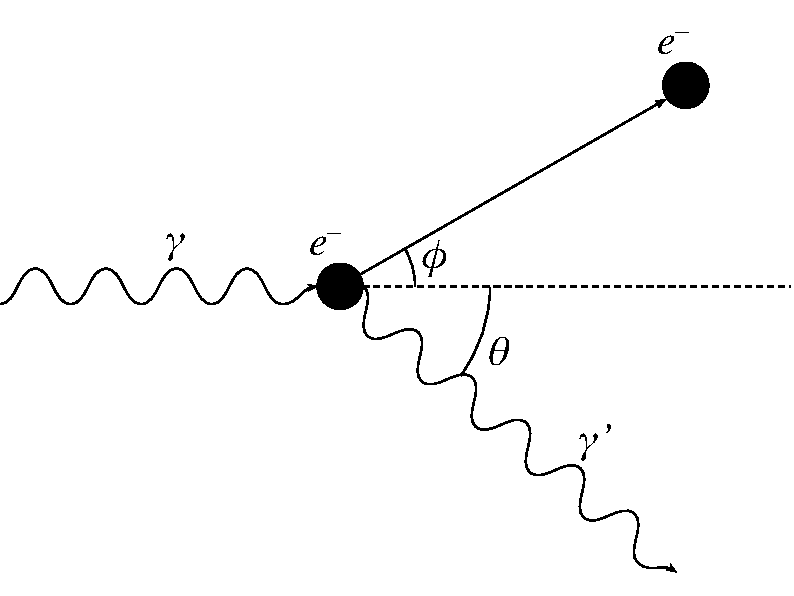
\includegraphics[width=.4\textwidth]{physical_aspects/Compton-scattering.pdf}
  \caption{\label{fig:Compton_scattering_diagram}Gamma-ray Compton scattering diagram.}
\end{figure}

Compton scattering osccurs most often when a photon interacts with an electron in the sensitive material, it can be understood as a colision between the two, where the electron is considered initialy static and then gains part of the photons energy $E_0$ after deflecting it. Fig \ref{fig:Compton_scattering_diagram} shows an example of a gamma ray being scattered by an electron, the recoil electron is ejected with an angle $\phi$ while the scattered gamma ray travels with an angle $\theta$. It can be shown that the energy of the scattered photon $E_{1}$ and the recoil electron $E_e$ follow equations \eqref{eq:compton}
\begin{align}
  E_{1} &= \frac{E_0}{1+\epsilon(1-\cos\theta)} \label{eq:compton},~ & E_e &= E_0 - E_1 = E_0\frac{\epsilon(1-\cos\theta)}{1+\epsilon(1-\cos\theta)};~ & \epsilon&=\frac{E_0}{m_{e}c^2} 
\end{align}
where $m_e c^2$ is the resting energy of the electron (511 \unit{\kilo\eV}). It is easy to see that high scattering angles greatly reduce the photon's energy, meaning that $E_e$ will be higher. For $\theta=\pi$ and $\phi=0$, it is therefore clear that the electron will gain the maximum energy possible, which is lower than $E_0$, this will be inportant while detecting gammas, since the photomultipliers collect the energy carried by electrons, which is further explored in Chapter \ref{chap:detection_methods}.

\subsubsection{Pair production}

This effect is the creation of a particle and its antiparticle from a neutral bosson, most often refer to when an electron and a positron are produced by a photon. In order for this to occur, the initial photon needs to have an energy higher to that of the resting pair ($2m_e c^2=1022$ \unit{\kilo\eV}), any exceding energy will turn into kinetic energy for the pair.

In the case of $^{22}$Na, as shown in Fig. \ref{sfig:22Na}, there is a transition from an excited state of $^{22}$Ne which emits a 1274.53 \unit{\kilo\eV} gamma, making pair production possible. Electron-positron annihilation is therefore a byproduct of this decay, making it important while studying its spectra.

\begin{figure}[H]
  \centering
  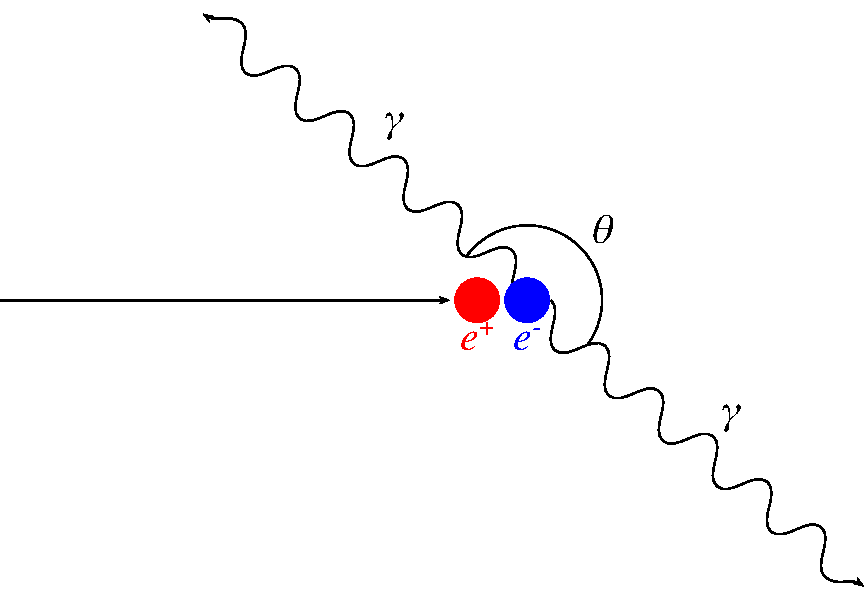
\includegraphics[width=.5\textwidth]{physical_aspects/positron-annihilation.pdf}
  \caption{\label{fig:positron_annihilation_diagram}Electron-positron annihilation diagram.}
\end{figure}

Once the positron produced by pair production slows down, it will most probably annihilate with an electron in the medium, producing two oppositely traveling gammas both with energy 511 \unit{\kilo\eV}, which combined is equal to the resting masses of both particles (1022 \unit{\kilo\eV}).

\section{Cosmic Radiation}



\section{Particle interactions with matter}